\documentclass{standalone}
\usepackage{amsmath}
\usepackage{amssymb}
\usepackage{mathtools}
\usepackage{bm}
\usepackage{tikz}
\usetikzlibrary{positioning}
\usetikzlibrary{calc}

\newcommand{\matr}[1]{\bm{#1}}
\newcommand{\vect}[1]{\bm{#1}}
\def\RSet{\mathbb{R}}

\definecolor{cb}{RGB}{32,32,32}
\definecolor{cbf}{RGB}{64,64,64}
\definecolor{cbt}{RGB}{64,64,64}
\definecolor{c1}{RGB}{204,204,255}
\definecolor{c2}{RGB}{204,255,204}

\tikzstyle{every neuron}=[cbt, circle, draw=cb, minimum size=1cm]
\tikzstyle{bias}=[cbt, circle,draw=cb]
\tikzstyle{operation}=[cbt, circle,draw=cb]
\tikzstyle{activation}=[cbt, draw=cb]
\tikzstyle{io}=[cbt]
\tikzstyle{sub}=[cbt]
\tikzstyle{subbox}=[cbt, draw=cb, fill=c2, rounded corners=1ex]
\tikzstyle{layer}=[cbt, draw=cb, fill=c1, minimum size=1cm, rounded corners=1ex]
\tikzstyle{delay}=[cbt, draw=cb,minimum size=0.5cm,fill=cbf, rounded corners=1ex]
\tikzstyle{neuron missing}=[draw=none, scale=4,text height=0.333cm,execute at begin node=\color{black}$\vdots$]
\tikzstyle{vmissing}=[draw=none, scale=4,text height=0.333cm,execute at begin node=\color{black}$\vdots$]
\tikzstyle{hmissing}=[draw=none, scale=4,text width=0.41cm,execute at
begin node=\color{black}$\cdots$]
\tikzstyle{line}=[cb, text=cbt]
\tikzstyle{arrow}=[cb, text=cbt, ->, >=stealth]
\tikzstyle{arrowInverse}=[cb, text=cbt, <-, >=stealth]
\tikzstyle{vectorLine}=[cb, text=cbt, line width=0.6mm]
\tikzstyle{vectorArrow}=[cb, text=cbt, ->, >=stealth, line width=0.6mm]
\tikzstyle{border}=[draw=cb, text=cbt]


\begin{document}
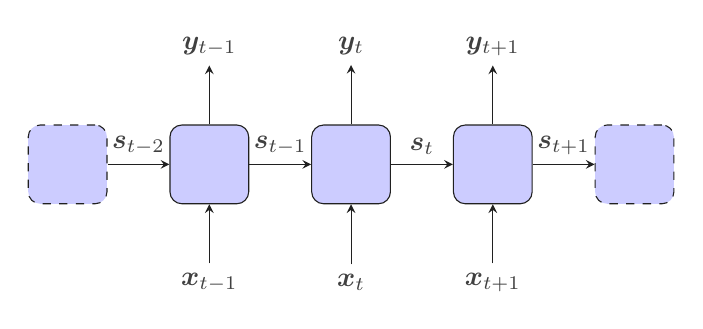
\begin{tikzpicture}[x=1.5cm, y=1.5cm]
  \foreach \l [count=\i] in {t-1,t,t+1}{
    \node [io] (input-\i) at (\i*1.2,0) {$\vect{x}_{\l}$};
    \node [layer] (state-\i) at (\i*1.2,1) {};
    \node [io] (output-\i) at (\i*1.2,2) {$\vect{y}_{\l}$};
    
    \draw [arrow] (input-\i) -- (state-\i);
    \draw [arrow] (state-\i) -- (output-\i);
  }
  \node [layer, dashed] (state-l) at (0,1) {};
  \node [layer, dashed] (state-r) at (4*1.2,1) {};
  
  \draw [arrow] (state-l) -- node[above]{$\vect{s}_{t-2}$} (state-1);
  \draw [arrow] (state-1) -- node[above]{$\vect{s}_{t-1}$} (state-2);
  \draw [arrow] (state-2) -- node[above]{$\vect{s}_{t}$} (state-3);
  \draw [arrow] (state-3) -- node[above]{$\vect{s}_{t+1}$} (state-r);
\end{tikzpicture}
\end{document}

